% --------------------------------------------------------------
% This is all preamble stuff that you don't have to worry about.
% Head down to where it says "Start here"
% --------------------------------------------------------------

\documentclass[12pt]{article}

\usepackage[margin=1in]{geometry} 
\usepackage{amsmath,amsthm,amssymb}
\usepackage{graphicx}

\newcommand{\N}{\mathbb{N}}
\newcommand{\Z}{\mathbb{Z}}

\newenvironment{exercise}[2][Exercise]{\begin{trivlist}
		\item[\hskip \labelsep {\bfseries #1}\hskip \labelsep {\bfseries #2.}]}{\end{trivlist}}
	
\makeatletter
\renewcommand*\env@matrix[1][*\c@MaxMatrixCols c]{%
	\hskip -\arraycolsep
	\let\@ifnextchar\new@ifnextchar
	\array{#1}}
\makeatother

\begin{document}
	
	% --------------------------------------------------------------
	%                         Start here
	% --------------------------------------------------------------
	
	%\renewcommand{\qedsymbol}{\filledbox}
	
	\title{Homework 3 (Due Sep 14, 2022)}%replace X with the appropriate number
	\author{Jack Hyatt\\ %replace with your name
		MATH 570 - Discrete Optimization - Fall 2022} %if necessary, replace with your course title
	
	\maketitle
	
	Justify all of your answers completely.
	
	\begin{exercise}{1} Solve the following LP using the simplex algorithm with tableaux, then verify your answer graphically.
		\begin{equation*}
			\begin{array}{ll@{}ll}
				\text{maximize}  & \displaystyle 3x_1+2x_2 &\\
				\text{subject to}& \displaystyle 2x_1+x_2 \leq 18   \\
				& \displaystyle 2x_1+3x_2 \leq 42 \\
				& \displaystyle 3x_1+x_2 \leq 24 \\
				& \displaystyle 0 \leq x_1,x_2
			\end{array}
		\end{equation*}
	\textbf{Answer}: The LP as a tableau is\\
	\[\begin{bmatrix}[ccccc|c]
		2 & 1 & 1 & 0 & 0 & 18\\
		2 & 3 & 0 & 1 & 0 & 42\\
		3 & 1 & 0 & 0 & 1 & 24\\
		3 & 2 & 0 & 0 & 0 & 0
	\end{bmatrix}\]
	The pivot element will be 1st column and 3rd row. Performing GE on this column results in
	\[\begin{bmatrix}[ccccc|c]
		0 & \frac{1}{3} & 1 & 0 & \frac{-2}{3} & 2\\
		0 & \frac{7}{3} & 0 & 1 & \frac{-2}{3} & 26\\
		1 & \frac{1}{3} & 0 & 0 & \frac{1}{3} & 8\\
		0 & 1 & 0 & 0 & -1 & -24
	\end{bmatrix}\]
	The next pivot element will be the 2nd column and 1st row. Performing GE on this column results in
	\[\begin{bmatrix}[ccccc|c]
		0 & 1 & 3 & 0 & -2 & 6\\
		0 & 0 & -7 & 1 & 4 & 12\\
		1 & 0 & -1 & 0 & 1 & 6\\
		0 & 0 & -3 & 0 & 1 & -30
	\end{bmatrix}\]
	The next pivot element will be the 5th column and 2nd row. Performing GE on this column results in
	\[\begin{bmatrix}[ccccc|c]
		0 & 1 & -\frac{1}{2} & \frac{1}{2} & 0 & 12\\
		0 & 0 & -\frac{7}{4} & \frac{1}{4} & 1 & 3\\
		1 & 0 & \frac{3}{4} & -\frac{1}{4} & 0 & 3\\
		0 & 0 & -\frac{5}{4} & -\frac{1}{4} & 0 & -33
	\end{bmatrix}\]
	This tell us that the optimal point is $x_1=3$ and $x_2=12$ with the optimal value being $33$.
	Here is the LP graphed with the obj function set equal to 33, as verification of the answer.
	\begin{center}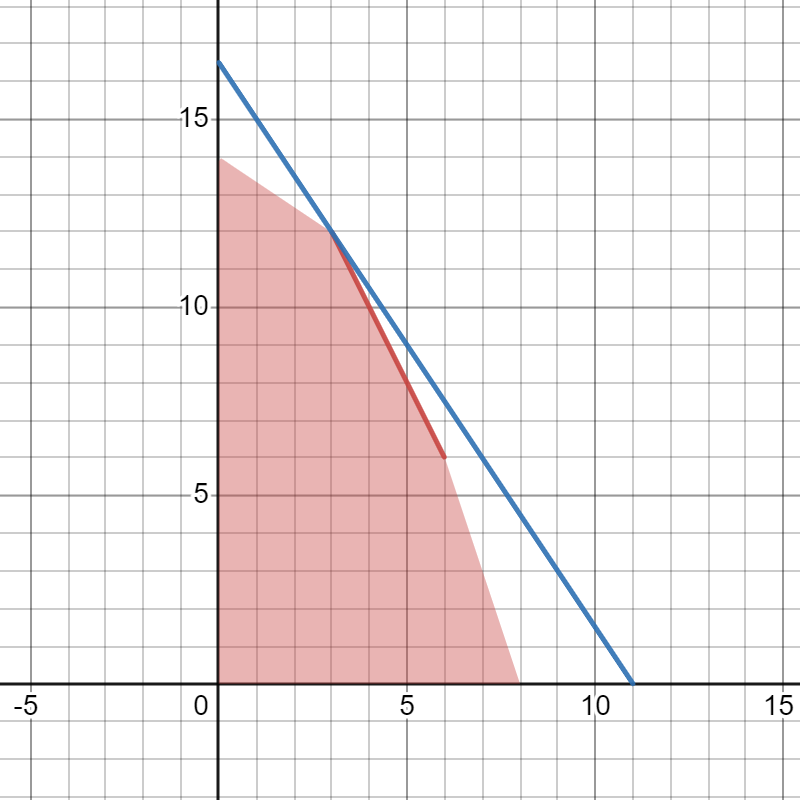
\includegraphics[scale=0.25]{desmos-graph}\end{center}
	\end{exercise}
	
	\begin{exercise}{2} Dualize the LP from Exercise 1, and then solve it.\\
		Since the primal in Exercise 1 was of the form
		\begin{equation*}
			\begin{array}{ll@{}ll}
				\text{maximize}  & \displaystyle \vec{c}^T\vec{x}\\
				\text{subject to}& \displaystyle A\vec{x} \leq \vec{b}\\
				& \displaystyle 0 \leq \vec{x}
			\end{array}
		\end{equation*}
		Then the dual will be of the form
		\begin{equation*}
			\begin{array}{ll@{}ll}
				\text{minimize}  & \displaystyle \vec{b}^T\vec{y}\\
				\text{subject to}& \displaystyle A^T\vec{y} \geq \vec{c}\\
				& \displaystyle 0 \leq \vec{y}
			\end{array}
		\end{equation*}
		So then the dual will be
		\begin{equation*}
			\begin{array}{ll@{}ll}
				\text{minimize}  & \displaystyle 18y_1 + 42y_2 + 24y_3 &\\
				\text{subject to}& \displaystyle 2y_1 + 2y_2 + 3y_3 \geq 3 \\
				& \displaystyle y_2 + 3y_2 + y_3 \geq 2 \\
				& \displaystyle 0 \leq y_1,y_2,y_3
			\end{array}
		\end{equation*}
		Since the dual is origin infeasible, my monkey brain doesn't know how to use the simplex method on this LP. Therefore, I must use the strong duality theorem, that uses the weak duality theorem, to say that since $\hat{x}$ solves the primal, $\hat{y}$ solves the dual. Looking at the last matrix in Exercise 1, the elements in the last row and in the 3rd through 5th columns are $-\hat{y}$. So $y_1 = \frac{5}{4}, y_2=\frac{1}{4}$, and $y_3=0$ minimizes the dual, which does produce 33 like the primal did.
	\end{exercise}
	
	\begin{exercise}{3} Solve the following LP.
		\begin{equation*}
			\begin{array}{ll@{}ll}
				\text{minimize}  & \displaystyle 2x+3y+4z &\\
				\text{subject to}& \displaystyle x + y + z \leq 10   \\
				& \displaystyle x \geq -3 \\
				& \displaystyle y \geq -5 \\
				& \displaystyle 3 \geq z \geq 0 \\
				& \displaystyle 4x - y - 2z = 2 \\
			\end{array}
		\end{equation*}
		Solving the equality for z and substituting it everywhere else yields us with
		\begin{equation*}
			\begin{array}{ll@{}ll}
				\text{minimize}  & \displaystyle 10x+y \\
				\text{subject to}& \displaystyle 3x + \frac{y}{2} \leq 11 \\
				& \displaystyle 4 \geq 2x-\frac{y}{2} \geq 1 \\
				& \displaystyle x \geq -3 \\
				& \displaystyle y \geq -5 \\
			\end{array}
		\end{equation*}
		Getting to (almost) standard forms looks like
		\begin{equation*}
			\begin{array}{ll@{}ll}
				\text{Let} &\displaystyle x=x'-3\\
				&\displaystyle y=y'-5\\
				\text{minimize}  & \displaystyle 10x'+y' \\
				\text{subject to}& \displaystyle 3x'+ \frac{y'}{2} \leq \frac{45}{2} \\
				& \displaystyle 2x' -\frac{y'}{2} \leq \frac{15}{2} \\
				& \displaystyle -2x' +\frac{y'}{2}\leq -\frac{9}{2} \\
				& \displaystyle 0 \leq x',y' \\
			\end{array}
		\end{equation*}
		This looks to not work with the simplex method on the primal (if I changed it to max, then the coeff would be negative and that messes it up), so therefore I will find the dual and use the simplex method on that.\\
		The dual in standard form will be 
		\begin{equation*}
			\begin{array}{ll@{}ll}
				\text{maximize}  & \displaystyle -\frac{9}{2}u+\frac{15}{2}v+\frac{45}{2}w \\
				\text{subject to}& \displaystyle -\frac{1}{2}u+\frac{1}{2}v-\frac{1}{2}w \leq -1 \\
				& \displaystyle 2u + 2v - 3w \leq -10 \\
				& \displaystyle 0 \leq u,v,w \\
			\end{array}
		\end{equation*}
		The LP as a tableau is\\
		\[\begin{bmatrix}[ccccc|c]
			-\frac{1}{2} & \frac{1}{2} & -\frac{1}{2} & 1 & 0 & -1 \\
			2  & 2 & -3 & 0 & 1 & -10  \\
			-\frac{9}{2} & \frac{15}{2} & \frac{45}{2} & 0 & 0 & 0  \\
		\end{bmatrix}\]
		The first pivot element will be 2nd col and 2nd row.
		\[\begin{bmatrix}[ccccc|c]
			-1 & 0 & 1/4 & 1 & -1/4 & 3/2 \\
			1 & 1 & -3/2 & 0 & 1/2 & -5  \\
			-12 & 0 & 45/4 & 0 & -15/4 & 75/2  \\
		\end{bmatrix}\]
		The next pivot element will be 3rd col and 1st row.
		\[\begin{bmatrix}[ccccc|c]
			-4 & 0 & 1 & 4 & -1 & 6 \\
			-5 & 1 & 0 & 6 & -1 & 4  \\
			33 & 0 & 0 & -45 & 15/2 & -30  \\
		\end{bmatrix}\]
		The simplex method has now ended. Looking at the last row, the two right most elements before the augment line gives us our answer for the primal.
	\end{exercise}
	
	\begin{exercise}{4} Solve the following LP, and provide the Gaussian-elimination matrix $G$ which, via left-multiplication, performs the full simplex algorithm on a tableau. Then, say what the record matrix R is.
		\begin{equation*}
			\begin{array}{ll@{}ll}
				\text{maximize}  & \displaystyle x+y+z &\\
				\text{subject to}& \displaystyle 0 \leq x \leq 1   \\
				& \displaystyle 0 \leq y \leq 1 \\
				& \displaystyle 0 \leq z \leq 1 \\
			\end{array}
		\end{equation*}
		The LP in standard form is 
		\begin{equation*}
			\begin{array}{ll@{}ll}
				\text{maximize}  & \displaystyle x+y+z &\\
				\text{subject to}& \displaystyle x \leq 1   \\
				& \displaystyle y \leq 1 \\
				& \displaystyle z \leq 1 \\
				& \displaystyle 0 \leq x,y,z
			\end{array}
		\end{equation*}
		
		The LP as a tableau is\\
		\[\begin{bmatrix}[cccccc|c]
			1 & 0 & 0 & 1 & 0 & 0 & 1 \\
			0 & 1 & 0 & 0 & 1 & 0 & 1 \\
			0 & 0 & 1 & 0 & 0 & 1 & 1 \\
			1 & 1 & 1 & 0 & 0 & 0 & 0 \\
		\end{bmatrix}\]
		By inspection, the optimal tableau (called $T_k$) will look like this
		\[\begin{bmatrix}[cccccc|c]
			1 & 0 & 0 & 1 & 0 & 0 & 1 \\
			0 & 1 & 0 & 0 & 1 & 0 & 1 \\
			0 & 0 & 1 & 0 & 0 & 1 & 1 \\
			0 & 0 & 0 & -1 & -1 & -1 & -3 \\
		\end{bmatrix}\]
		And $T_k$ has this form
		\[\begin{bmatrix}[cc|c]
			RA & R & R\vec{b} \\
			\vec{c}^T-\hat{y}^TA & -\hat{y}^T & -\hat{y}^Tb \\
		\end{bmatrix}\]
		and by inspecting $T_k$, we see that R is the same as the 3x3 identity matrix.\\
		G has the form
		\[\begin{bmatrix}
			R & \vec{0} \\
			-\hat{y}^T & 1 \\
		\end{bmatrix}\]
		and equals
		\[\begin{bmatrix}[cccccc|c]
			1 & 0 & 0 & 0 \\
			0 & 1 & 0 & 0 \\
			0 & 0 & 1 & 0 \\
			1 & 1 & 1 & 1 \\
		\end{bmatrix}\]
		
	\end{exercise}
	
	% --------------------------------------------------------------
	%     You don't have to mess with anything below this line.
	% --------------------------------------------------------------
	
\end{document}

\begin{equation*}
	\begin{array}{ll@{}ll}
		\text{minimize}  & \displaystyle\sum\limits_{j=1}^{m} w_{j}&x_{j} &\\
		\text{subject to}& \displaystyle\sum\limits_{j:e_{i} \in S_{j}}   &x_{j} \geq 1,  &i=1 ,..., n\\
		&                                                &x_{j} \in \{0,1\}, &j=1 ,..., m
	\end{array}
\end{equation*}
